\documentclass[referee, 
	            sn-basic]
           {sn-jnl}

\usepackage{lineno,hyperref}
\usepackage{longtable, booktabs, amsmath, textcomp}
\usepackage{natbib}

% Put Abstract on new page to create title page as per Oecologia guidelines
	\usepackage{etoolbox}
	\pretocmd{\abstractname}{\newpage}{}{}

% Springer stuff 
\jyear{2022}%
\raggedbottom
\unnumbered% uncomment for unnumbered level heads

\begin{document}
\raggedright

\title[Rangeland grasshoppers and prescribed fire]{Attracted by higher crude protein, grasshopper abundance and offtake increase after prescribed fire}


\author*[1]{\fnm{Nicholas Gregory}  \sur{Heimbuch}}\email{ngh11@pitt.edu}

\author[2]{\fnm{Devan Allen} \sur{ McGranahan}}\email{Devan.McGranahan@usda.gov}
\author[3]{\fnm{Carissa L.} \sur{ Wonkka}}\email{Carissa.Wonkka@usda.gov }
\author[2]{\fnm{Lance T.} \sur{Vermeire}}\email{Lance.Vermiere@usda.gov}
\author[3]{\fnm{David H.} \sur{Branson}}\email{Dave.Branson@usda.gov }

\affil*[1]{\orgname{University of Pittsburgh}, 
	                  \orgaddress{\street{4200 Fifth Ave}, 
            		     \city{Pittsburgh},
            		     \postcode{15260}, 
           		     \state{Pennsylvania},
            		     \country{USA}}}

\affil[2]{\orgname{USDA Agricultural Research Service}, 
	     \orgdiv{Livestock \& Range Research Laboratory},
              \orgaddress{\street{243 Ft. Keogh Rd.}, 
            		     \city{Miles City},
            		     \postcode{59301}, 
           		     \state{Montana},
            		     \country{USA}}}
\affil[3]{\orgname{USDA Agricultural Research Service}, 
	     \orgdiv{Northern Plains Agricultural Research Laboratory},
              \orgaddress{\street{1500 N Central Ave}, 
            		     \city{Sidney},
            		     \postcode{59270}, 
           		     \state{Montana},
            		     \country{USA}}}
         		     
\clearpage

\abstract{Grasshoppers are critical components of open ecosystems, such as grasslands and savannas, worldwide. 
While often seen as pest species competing with domestic livestock for forage resources and damaging crops, many species never reach abundances that result in economic damage and can provide essential ecosystem services. 
Grasshopper population and community dynamics are modulated by the processes that determine plant structural and community dynamics in a given ecosystem; in open ecosystems, fire is one of the most ubiquitous. 
This study examined how indirect fire effects (improved forage quality) affect the density of and offtake by grasshoppers at two different times since fire and in unburned plots.
Both offtake and density were significantly higher in burned plots compared to unburned plots.
Burned plot grasshopper density increased over time, with greater rates of increase in recently burned plots, while density remained constant in unburned locations.
These density and offtake patterns appear to be the result of higher crude protein content in burned plots, on account of them having a much higher proportion of recent growth after fire removed aboveground senesced material. 
These findings present a mechanism by which fire interacts with grasshopper abundance and distribution in open ecosystems. 
Long term assessments of fire and its interaction with grazing and weather patterns are necessary to determine if attraction to and consumption of post-fire vegetation will result in greater performance of pest grasshopper species or enhance community diversity, regulating pest species outbreaks.} 

\keywords{Fire-grazing interaction; Magnet effect; Orthoptera: Acrididae; Prescribed fire; Pyric herbivory; Rangeland forage quality; Rangeland pest management}

\maketitle
\begin{linenumbers}

\section{Introduction}

As globally-ubiquitous herbivores, grasshoppers (Orthoptera: Acrididae) contribute to ecosystem function around the world. 
Historically, interest in grasshoppers has generally increased with their local density, as grasshopper outbreaks and locust swarms have wrought economic damage for centuries \citep{cease2015}. 
While such outbreaks were long considered to be primarily driven by environmental conditions beyond human control, research has described close interactions between land management and grasshopper dynamics \citep{legall2019}. 
Although the utility of this broader understanding of grasshoppers and human land use has mostly been realized within the context of pest control \citep{branson2006}, grasshoppers also contribute to ecosystem dynamics including nutrient cycling and plant community composition \citep{meyer2002,zhang2011,kietzka2021, belovsky2000}. 

Grasshoppers are particularly important in \emph{open ecosystems}\textemdash rangeland biomes such as grasslands and savannas because herbaceous plant communities are regulated by frequent disturbances and their interaction, especially herbivory and fire \citep{bond2022}. 
Interactions between grasshoppers, fire, and other herbivores drive interconnected plant, nutrient, and soil microbial dynamics, impacting ecosystem services derived from open ecosystems.
For instance, grasshoppers are widely seen as pests in competition with economically-valuable livestock for herbaceous primary productivity \citep{zhang2019}. 
\citet{hewitt1983} estimated grasshoppers consume nearly US\$400 million (US\$1.7 billion inflation-adjusted) worth of livestock forage per year in the western United States.  
Meanwhile, fire interacts with grasshoppers via direct and indirect effects, which are variable among species depending on their biology \citep[e.g.][]{vermeire2004}. 
Direct effects include mortality of adults and eggs from heat exposure, while indirect effects include alterations to host plant availability, vegetation structure, and microclimate.
Thus the fire-grasshopper interaction also has implications for grasshopper-livestock competition. 

Because the nutritive value of vegetation in open ecosystems often varies depending on the time since it last burned, fire likely also affects grasshoppers by modulating their food resources. 
Perennial, fire-adapted plants resprout using energy stored in organs protected from heat damage, and post-fire plant tissue is typically higher in crude protein and lower in structural carbohydrates than the mature or senescent tissue that was consumed by the fire \citep{mcgranahan2021}. 
Thus, despite overall lower plant biomass on account of the fire, grasshopper abundance on recently-burned areas is often higher than unburned areas, especially for graminivorous (grass-eating) species \citep{meyer2002}. 
More broadly, post-disturbance succession and plant nutritive value have been identified as important factors in grasshopper abundance \citep{fartmann2012, schirmel2019}. 
Yet explicit examinations between time-since-fire, plant nutritive value, and grasshopper abundance have not been conducted. 

We measured grasshopper abundance and forage consumption, along with grass protein content, in a replicated experiment that created a time-since-fire gradient in temperate grassland.  
Because grasshoppers are morphologically capable of much more precise herbivory than most vertebrate grazers, we measured protein content of grass leaves and stems separately.
We predicted that more-recently burned plots would have both higher protein content\textemdash especially in leaves\textemdash and greater grasshopper abundance. 
As such, we predicted a greater degree of vegetation removal by grasshoppers from recently-burned plots, as determined by comparing aboveground plant biomass against that from within grasshopper exclosures. 

\section{Methods}

\subsection{Study location \& design} 

Our study was conducted at the USDA-Agricultural Research Service Livestock and Range Research Laboratory in Miles City, Montana, USA (46.40 N, 105.95 W).  
Vegetation is typical mixed-grass prairie, and the study site was dominated by western wheatgrass \emph{Pascopyrum smithii}.  
The overwhelming majority of grasshoppers on the study site, as determined by mid-season sweep netting and identification at the USDA-ARS Pest Management Research Unit in Sidney, Montana, consisted of the migratory grasshopper \emph{Melanoplus sanguinipes}, a native species of spur-throated grasshopper in the family Acrididae. 

Within a larger prescribed fire experiment, we selected nine, 300-m\textsuperscript{2} plots to test three different time-since-fire treatments (n=3 each): Fire the previous autumn, fire the previous spring, and a control treatment left unburned for several years. 
Livestock were excluded from the entire study area and had been for several years.
While the study area was open to wildlife such as deer \emph{Odocoileus} spp., pronghorn \emph{Antilocapra americana}, and lagomorphs including \emph{Sylvilagus floridanus} and \emph{Lepus} spp, we observed no evidence of their presence on any plots during the sampling period. 

\subsection{Sample collection}

To measure the amount of vegetation removed by foraging grasshoppers, we established two pairs of sample points within each plot. 
Each pair of 0.25-m\textsuperscript{2} sample points consisted of one full mesh grasshopper exclosure alongside another structure with a similar footprint and shade factor that was open to grasshopper herbivory.
Each type of structure consisted of a polyvinyl chloride tube frame with heavy nylon netting, which when fully wrapped and zipped around the frame and weighted down with sand-filled tubes, effectively kept grasshoppers out \citep{parker1985}. 
Because the mesh reduced sunlight intensity by 400 w m\textsuperscript{-2} compared to the
surrounding area, we designed control structures that remain open on the north and south faces to allow grasshoppers to enter while still producing shade conditions that matched the exclosures during peak photosynthetic activity. 
These paired structures ensured that shade would not influence grass development, skewing offtake measurements. 
Structures were monitored at least every 48 hr and after any substantial weather event to ensure they remained intact; in the few instances grasshoppers had crawled under the exclosures, they were removed upon discovery. 

On all plots, the first pair of structures was established 1 July 2021, and the second pair 1 week later. 
On 9 August\textemdash 40 d after the first pair of structures were erected\textemdash 
all aboveground biomass, standing dead and current year's growth, within each 0.25 m\textsuperscript{2} frame footprint was clipped to ground level.
Within the recently-burned plots, individual grass tiller counts were recorded\textemdash because structures were placed randomly and tiller density was observed to be variable, we prepared to express biomass on both a per-tiller basis as well as by area. 
Clipped biomass was dried at 60$^\circ$C for 48 hr and weighed to the nearest 0.001 g. 

%I checked every exclosure routinely for grasshopper breaches with no
%more than 48 hours elapsing between examinations. The large margin of
%error in our spring burn offtake is likely due to an exclosure breach
%that occurred on July 19th, 19 days into the experiment timeline. After
%a 48 hour break between quality checking the exclosures I noticed a
%number of grasshoppers had made it into the exclosure after it sustained
%storm damage, so grasshoppers could have been actively foraging in the
%exclosure for a maximum of two days. Although this was a short period of
%possible contamination, this is the most likely cause for the wide
%margin of error. There was no statistical difference in offtake rate
%between spring and fall burn treatments. After 40 days, on August 9th,

We collected forage quality samples on the 26th day of the study, roughly halfway through the study period.
For each plot, samples were comprised of 40 western wheatgrass tillers randomly selected by tossing a marker flag in the air and clipping, to ground level, the tiller nearest to where it landed, regardless of phenology or live/dead status. 
Tillers were  separated into leaf blades and stems (which included leaf sheaths) prior to drying at 60$^\circ$C for 48 hr and grinding into fine powder. 
Protein content was determined with a Thermo Scientific Flash 2000 combustion analyzer. 

To determine grasshopper density, we employed a standard ring count methodology
\citep{onsager1977, joern2013}. 
One week after the initial pairs of structures were established, we placed 5, 0.1 m\textsuperscript{2} rings on the ground in a {\large{$\times$}} pattern centered on each plot, with rings approximately 1.5 m apart and at least 2 m from plot edges.
Nineteen observations were made over the course of the study period, between 9 July and 6 August. 
All plots were sampled in each round of observations by a single observer (N.G.H.), and all observations were conducted between 1000 and 1200 for consistent solar conditions. 
Sampling consisted of walking slowly through the plot and agitating the area near each ring with a long stick, and recording the number of grasshoppers that jumped from the ring.

\subsection{Data analysis}

To determine whether accessibility to grasshoppers affected the amount of aboveground vegetation, we subtracted the dried biomass values from control structures from that of their paired grasshopper exclosures and calculated the mean of these two differences for each plot (n = 3 experimental units per treatment). 
To account for the different lengths of deployments among the two pairs of structures, offtake was expressed as daily rate of removal by dividing the difference in biomass between paired structures by the number of days each structure pair was deployed.  
We used a linear model with the intercept term removed to test each of the three difference values against 0 (null hypothesis: no difference in standing crop between grasshopper exclosures and control frames) using the \texttt{lm} function in the \textsf{R} statistical environment \citep{Rcore2020}. 
We tested pairwise contrasts in standing crop differences across each treatment with a post-hoc Tukey test using \texttt{TukeyHSD}.

We determined whether crude protein content varied with fire treatment and plant organs (leaf blades vs. stems) by fitting each term and their interaction in an ANOVA.
Pairwise contrasts among fire treatments were again tested with \texttt{TukeyHSD}.

To determine if there were general linear trends in grasshopper abundance patterns over the course of the study, we conducted a nonparametric test of the Kendall's tau (\(\tau\)) statistic fit to the grasshopper count data within each burn treatment using the \texttt{kendallTrendTest} function in the \emph{EnvStats} package for
\textsf{R} \citep{millard2013}.
To compare the relative rates of change over the study period, we plotted the estimated slope of the trend for each burn treatment and the associated 95\% confidence intervals as returned by \texttt{kendallTrendTest}.

\section{Results}

\begin{figure}
\centering
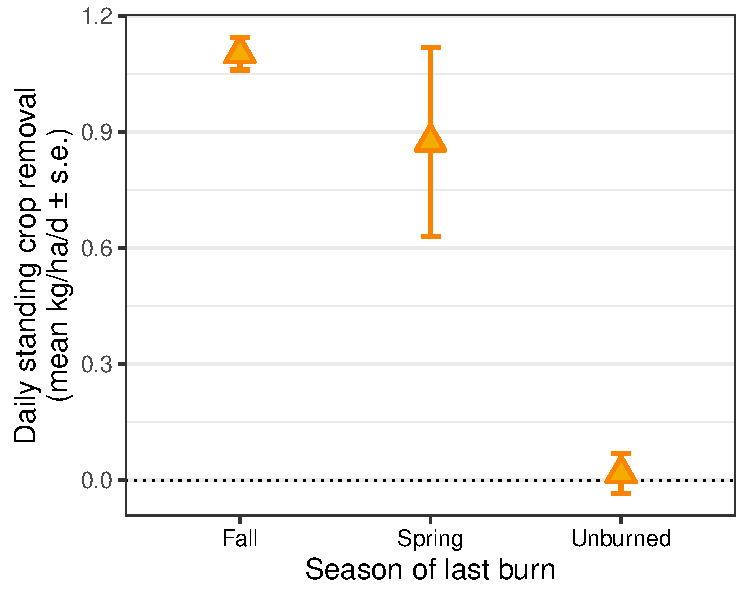
\includegraphics{removal_gg-1.pdf}
\caption{Mean differences in biomass removal rate between grasshopper exclosures and control frames in plots with three different fire treatments. 
Standing crop was determined by clipping at the end of the four-week study period and differences attributable to grasshopper removal are expressed as mean kg ha\textsuperscript{-1} day\textsuperscript{-1}.}
\label{removal} % Fig.~\ref{removal}
\end{figure}

Overall, aboveground plant biomass was lower outside of exclosures in both fire treatments (64 $\pm$ 4\% less in fall burn plots and 55 $\pm$ 9\% less in spring burn plots), but did not differ between exclosures and accessible unburned plots (1 $\pm$ 8\%).
Biomass removal by grasshoppers accounted for statistically-significantly lower biomass outside of grasshopper exclosures in both fall and spring burns (\(t =\) -7.6,
\(P\) \textless{} 0.001 and \(t =\) -6, \(P\) \textless{} 0.001, respectively).
But there was no difference in offtake among spring and fall burns (\(P\) \textgreater{} 0.05), with grasshoppers removing approximately 1.0 ($\pm$ 0.2) kg ha\textsuperscript{-1} d\textsuperscript{-1} in each (Fig.~\ref{removal}). 
Aboveground biomass was not different between grasshopper exclosures and areas accessible to grasshoppers in unburned plots (\(t =\) -0.12, \(P\) \textgreater{} 0.05).
 Offtake was significantly lower in unburned plots than plots burned in both the previous fall and spring (\(P\) \textless{} 0.01 and \(P\) = 0.01, respectively).

\begin{figure}
\centering
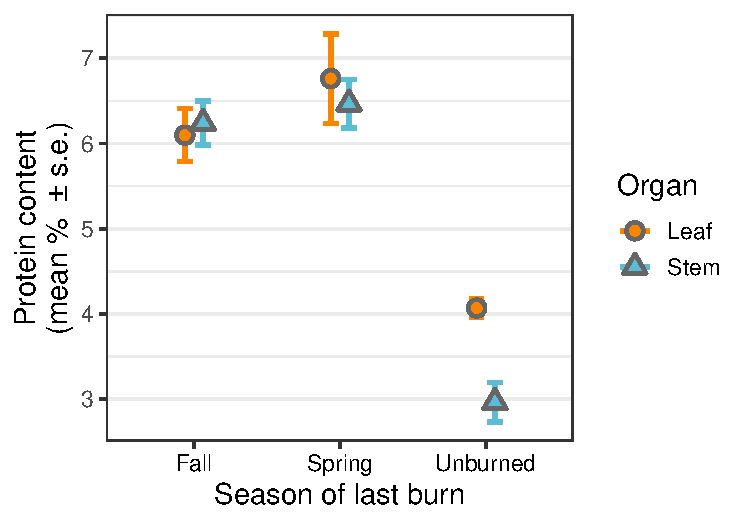
\includegraphics{value_gg-1.pdf}
\caption{Mean protein content of western wheatgrass \emph{Pascopyrum smithii} sampled from three burn treatments as a percentage of total dry matter. 
Orange circles indicate the protein content of leaf blades; blue triangles are stems (which include leaf sheaths).}
 \label{value} % (Fig.~\ref{value})
\end{figure}

Crude protein content varied among the fire treatments (\(t =\) 57, \(P\) \textless{} 0.001; Fig.~\ref{value}). 
Crude protein content in fall and spring burns averaged 6.4\% ± 0.2 s.e. and did not differ from one another (\(P\) \textgreater{} 0.05). 
But crude protein content in unburned  plots\textemdash which included a substantial amount of senesced material from previous growing seasons\textemdash was lower than in both fall and spring burns plots (\(t =\) -2.7, \(P\) \textless{} 0.001 and \(t =\) -3.1, \(P\) \textless{} 0.001, respectively).

Across all samples, crude protein content did not vary among leaves and
stems (\(t =\) 2.7, \(P\) \textgreater{} 0.05). Despite a trend towards
higher crude protein in leaf tissue in unburned plots (Fig.~\ref{value}), the
pattern was not influential enough to create a significant fire
treatment \(\times\) organ interaction (\(t =\) 2.1, \(P\)
\textgreater{} 0.05).

\begin{figure}
\centering
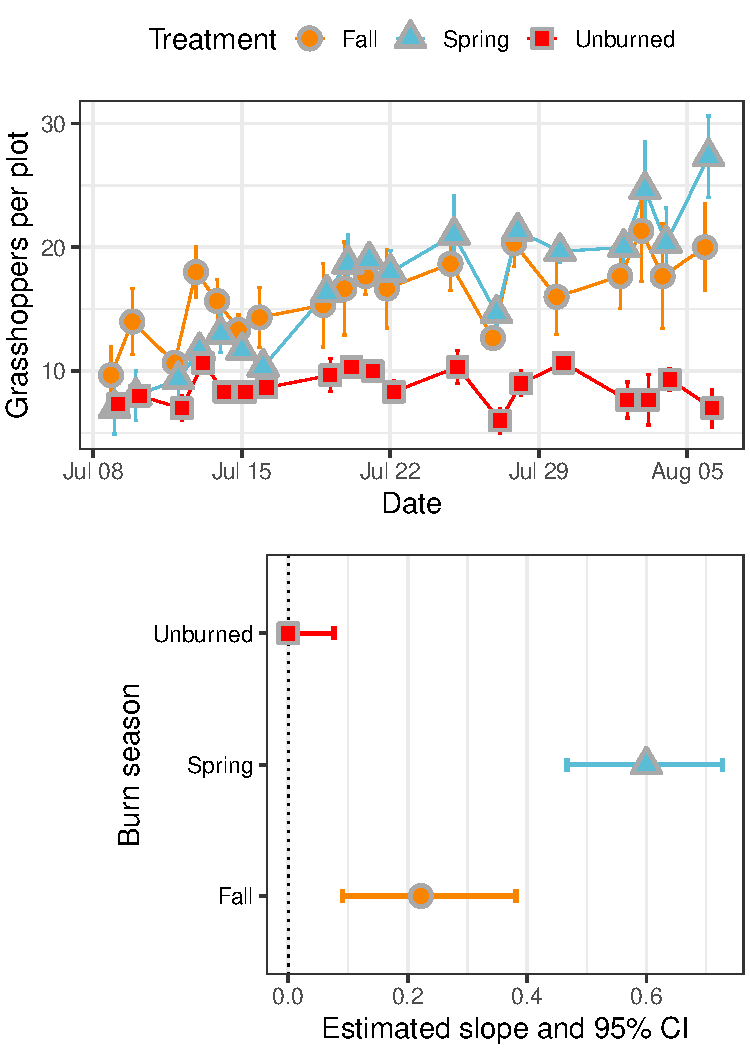
\includegraphics{tau_gg-1.pdf}
\caption{Observed grasshopper counts per square meter. 
Orange indicates data taken from fall burn treatments, blue from spring burn treatments, and red from unburned (control) plots.
\emph{Bottom} shows data from Kendall's Tau statistic which assessed the observed count trendline consistency over time. 
Our tau values were compared against the null hypothesis that there was no trend in our data. 
95\% confidence intervals were calculated to show the possible variance in slope for the data over time. 
Most grasshoppers observed were the migratory grasshopper \emph{Melanoplus sanguinipes}.}
\label{tau} % Fig.~\ref{tau}
\end{figure}

Grasshopper abundance was similar across plots at the beginning of the study period (early July) but increased significantly over the next month in fall and spring burn plots (\(\tau =\) 0.29, \(P\) \textless{} 0.01 and \(\tau =\) 0.62, \(P\) \textless{} 0.001; Fig.~\ref{tau}). 
Grasshopper abundance remained constant over the study period in unburned plots (\(\tau =\) 0.039, \(P\) \textgreater{} 0.05). 
While grasshopper abundance increased in both burn treatments, the rate of increase was approximately three times greater in plots that had been most recently burned in the spring than those that had been burned in the previous fall (Fig.~\ref{tau}, \emph{bottom}), which represented more than a five-fold increase in density from approximately 5 to 25 grasshoppers m\textsuperscript{-2} (Fig.~\ref{tau}, \emph{top}).

\section{Discussion}

Insect herbivore abundance and distribution are extremely spatially and temporally variable \citep{cappuccino1995}. This variability is often tied to variability in plant biomass and nutrient content \citep{joern2012}. Insect herbivores often select plant species or suites of species based on specific nutritional needs \citep{ibanez2013, behmer2008} and will actively seek a diet that contains a specific ratio of nutrients \citep{behmer2009}. Therefore, the distribution of plant nutritional quality on the landscape can be a strong determinant of grasshopper abundance and distribution \citep{white2012, joern2012, ozment2021}. 

In the present study, grasshoppers removed over half of available biomass over the study period in burned plots but had no detectable effect in unburned plots. This is likely related to crude protein content which was elevated in burned plots and the resultant increase in grasshopper abundance over time in plots that had been burned in either the spring or previous fall. Grasshoppers in other systems have been shown to select burned vegetation: grasshoppers feeding in willow selected resprouting burned willow shoots, consuming them completely, while rejecting unburned willow after a taste \citep{stein1992} and in the Brazilian Cerrado, leaf chewing insects including grasshoppers selected resprouting burned shrubs, causing 30-60 percent greater damage to resprouting leaves than unburned leaves \citep{lopes2011}. 

Time since last fire is a driver of spatial and temporal variability in the distribution of plant nutritional quality. Resprouting plant tissues typically have higher protein content than their mature counterparts on account of having a lower proportion of structural carbohydrates \citep{mcgranahan2021}. 
At the stand level, fire removes low-quality, senesced material from previous season's growth, allowing high-quality regrowth to dominate the sward.  
This elevated protein content in burned areas can be maintained over longer periods by repeated grazing \citep{wanchuk2021}, even during drought \citep{spiess2020}. 
Higher nutritional quality attracts herbivores to an area after fire and they maintain the high nutritional quality by remaining in that area to continue consuming high quality plant tissues that must then regrow and this feedback has been documented for a range of herbivores in open ecosystems worldwide \citep{allred2011, archibald2005, sensenig2010}. 
The dominant grasshopper species in our plots, \emph{Melanoplus sanguinipes}, shows preference for current year's growth and standing dead material makes up only a small proportion of its diet \citep{anderson1952, mulkern1962}.
In the present study, burned plots with overall higher crude protein content as a result of higher proportions of resprouting, green tissue, attracted \emph{M. sanguinipes} from surrounding unburned vegetation.


In this study, the rate of increase in grasshopper abundance was greater in spring burn plots, which were burned most recently. Although there were no differences in absolute abundance between fall and spring burn plots, the differences in rate of increase over the course of the study suggests that divergence of grasshopper abundance between spring and fall burned plots likely became significant by the end of the growing season. This points to a fire-grazing nutrient feedback \textemdash the most recently burned plots maintained that strong feedback over the course of the study while the attraction was not as strong to fall burn plots. Crude protein content did not differ between fall and spring burn plots at the time it was measured \textemdash halfway through the study in mid July. However, given the differential rate of increase in spring and fall burn plots, crude protein between those treatments likely diverged later in the growing season, along with grasshopper abundances. 

%Other studies finding an increase in insect herbivore abundance in burned vegetation reference the plant vigor hypothesis. The plant vigor hypothesis describes improved colonization, establishment, survival, and even reproductive rates for herbivores consuming rapidly growing plant tissue \citep{price1991}. This is attributed to enhanced nutritive value or a reduction in antiherbivory secondary metabolites. For instance, leaf galling insect abundance and larvae survival were higher on more nutritive regrowth following fire than in unburned Cerrado \citep{vieira1996} and increased leaf nitrogen content after fire corresponded with higher abundance of canopy arthropods due to enhanced colonization and survival than in unburned eucalyptus \citep{radho-toly2001}. 

Grasshopper population dynamics and resultant community composition are impacted by many drivers simultaneously. In addition to plant nutritional status, predation risk \citep{schmitz1997}, dispersal limitation \citep{hawlena2010}, and microclimatic conditions \citep{bauer2007, gardiner2008} are strong determinants of grasshopper dynamics. Because of the role it plays in each of these, vegetation structure often correlates with grasshopper distribution and density, although the strongest correlations have occurred in highly productive grasslands such as tallgrass prairies \citep{joern2004}. In the present study, fire altered both vegetation nutritional status and structure, making it difficult to parse which drove increases in grasshopper abundance. And both likely play some roll in driving grasshopper habitat selection. The dominant species found during our study has been shown to respond positively to nitrogen in this ecosystem \citep{branson2003}. In addition, grasshoppers showed similar attraction to high nutrient grazing lawns in tallgrass prairie \citep{ozment2021}. While there is a similar conflation of structure and nutrient content to that in the present study, they found the attraction weaker when the nutritional contrast between grazing lawns and surrounding areas lessened during drought, supporting nutritional quality as an important driver. Regardless of the mechanism, recently burned plots clearly attracted more grasshoppers and subsequently had more aboveground biomass removal than unburned plots, which has potential implications for management. 

%In addition, the dominant species in the present study is a mixed feeder, which are typically less responsive to changes in plant nitrogen \citep{joern2012, jonas2008}. However, given that our study was conducted during the hot summer months during a drought, grasshoppers would likely seek taller stature vegetation to facilitate thermoregulation rather than the shorter stature vegetation of the burned plots. And mixed feeders are thought to be less responsive to changes in plant nitrogen content because they are able to maintain preferred nutrient ratios by consuming both nitrogen-rich forbs and lower-nitrogen grasses \citep{jonas2008}. In the present study, previous management resulted in low forb density, which was exacerbated by drought, potentially forcing even mixed feeders to seek the higher crude protein content of recently burned vegetation. 

Because grasshoppers can be economic pests in grasslands used for livestock production when at high densities, improved survival and reproduction resulting from nutrient enhancement in burned vegetation \citep{branson2003} could intensify competition between livestock and grasshoppers in burned areas. Loss of livestock forage to grasshoppers is most problematic during grasshopper outbreaks or during droughts, when plant productivity is low \citep{belovsky1995, joern2000, branson2014}. 
The dominant grasshopper at our study area, the migratory grasshopper \emph{Melanoplus sanguinipes}, is commonly viewed as one of the most frequent economic pest species in the central and western US, making it especially damaging to farmers and ranchers throughout the Great Plains \citep{onsager2000a, olfert2021}. 
However, many grasshopper species do not cause economic harm and instead enhance ecosystem service delivery by increasing nutrient cycling, providing food for rangeland wildlife, exerting some control over unwanted rangeland plants, and in some cases increasing overall rangeland productivity \citep{branson2006}. In addition, greater grasshopper diversity can reduce the likelihood of pest species outbreaks as beneficial grasshoppers compete for resources and enhance the efficacy of grasshopper predators \citep{branson2006}. Fire at appropriate scales could enhance diversification of grasshopper communities because they exhibit a breadth of species-specific habitat requirements and fire can enhance structural and nutritive heterogeneity in vegetation. 

Gains in grasshopper performance from nutritive enhancement could be offset by negative fire effects, as fire alone can result in short-lived reductions in grasshopper abundance by up to 75\% \citep{branson2016}, although the effects are often short-lived. 
Direct effects of fire include adult and nymphal mortality \citep{bock1991}, and egg mortality due to soil heating \citep{branson2013, branson2016, vermeire2004}. 
Indirect effects related to microclimate, soil properties, and plant community compositional changes can also alter grasshopper abundance in burned areas \citep{vanwingerden1991,schirmel2011, evans1983,matenaar2014, meyer2002}, although other drivers, such as livestock grazing, likely interact with fire in most grasslands \citep{mcgranahan2021,fuhlendorf2009,joern2005}. Given these wide-ranging impacts on diversity and mortality, fire could be a sustainable low-cost alternative to conventional control of economically-damaging grasshopper outbreaks \textemdash broad-scale chemical applications \citep{branson2006}, which are expensive, unreliable, and have non-target effects on beneficial arthropods. In addition, ecosystem services provided by non-pest grasshopper species are lost when insecticides are used to control grasshopper outbreaks \citep{joern2000}. Longer-term assessment of grasshopper dynamics in burned and unburned areas is needed to determine the potential for fire to reduce outbreaks of economically damaging grasshopper species.  

Future research should also assess the impacts of fire at larger scales and the interaction of fire with other disturbances such as drought and livestock grazing. Grasshopper responses observed in this study likely reflect movement patterns and attraction to burned plots, which might differ at large scales. Studies of fire-herbivore feedbacks at multiple scales show that small-scale fires result in positive feedbacks, creating grazing hotspots with high crude protein for long durations, similar to our findings here\citep{cromsigt2008}. In contrast, large-scale fires can result in more dispersed herbivore distribution that can homogenize plant nutritional status and structure as grazing pressure is dispersed, resulting in more ungrazed areas within a burn perimeter that do not maintain high nutrient content \citep{archibald2005} and lessening the attraction of the burned area to herbivores \citep{donaldson2018}. However, it is uncertain whether heterogeneity in protein content distribution within a broader fire could result in the creation of similar small-scale nutrient hotspots in the presence of grasshoppers or if the additional grazing pressure from grasshoppers could enhance livestock attraction to burned areas at larger scales. Regardless of scale, livestock grazing-fire interactions \citep{onsager2000a, oneill2003} and drought likely play a role in fire-grasshopper dynamics by either enhancing or diminishing contrast in protein content between unburned and burned vegetation \citep{augustine2014, yoganand2014, ozment2021}, and our findings suggest that this contrast is an important driver of grasshopper distribution and offtake. 



\backmatter


\bmhead{Acknowledgments}

We appreciate the general assistance of D.F. Watson from NPARL in organizing field equipment, the assistance of Cheryl Murphy, with protein analysis at LARRL, and Nicole Davidson, with grasshopper identification at NPARL. 


\bmhead{Conflict of Interest} 

The authors declare that they have no conflict of interest.

\bmhead{Funding} 

NGH received salary support from the USDA-ARS Plains Area co-funded internship with matching funds from LARRL and NPARL. 

\bmhead{Ethics statement} 

This article does not contain any studies with human participants or animals performed by any of the authors.  

\bmhead{Availability of data and code}

Data and \textsf{R} script used herein are available under a U.S. Public Domain license at the USDA Ag Data Commons (\href{doi.org/10.15482/USDA.ADC/1528475}{https://doi.org/10.15482/USDA.ADC/1528475}). 

\bmhead{Author contributions}

\emph{This Highlighted Student Paper represents a novel approach to both fire-grazing interaction research\textemdash by focusing on invertebrate herbivores in an ungulate-dominated ecosystem\textemdash and research on fire effects on grasshoppers\textemdash most grasshopper research focuses on direct fire effects on grasshopper mortality.} 

NGH collected data. 
NGH and DAM analyzed data. 
NGH wrote the initial draft of the paper, which DAM and CLW edited with input from LV and DB.
LV was responsible for the prescribed fire treatments from which data were collected. 
DB provided grasshopper expertise and sampling equipment.

\bibliography{HopperzBib.bib}

\end{linenumbers}
\end{document} 